
\begin{figure*}[!th]
	\centering

	\begin{tabular}{@{}r@{ } c@{ } c@{ } c@{ } c@{ } c }
	&
	\small{-0.00 D} &
	\small{-1.00 D} &
	\small{-2.00 D} &
	\small{-3.00 D} &
	\small{-4.00 D} & \\

	\begin{sideways} \parbox[b]{20mm} {Camera} \end{sideways} &
	
\includegraphics[width=0.185\textwidth]{../../__Images/05/WB_N(20-200)_-0D_to_-4D/wb_N_20-200_Camera-0,00D(lens).png} &
	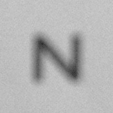
\includegraphics[width=0.185\textwidth]{../../__Images/05/WB_N(20-200)_-0D_to_-4D/wb_N_20-200_Camera-1,00D(lens).png} &
	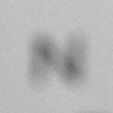
\includegraphics[width=0.185\textwidth]{../../__Images/05/WB_N(20-200)_-0D_to_-4D/wb_N_20-200_Camera-2,00D(lens).png} &
	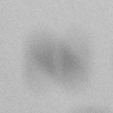
\includegraphics[width=0.185\textwidth]{../../__Images/05/WB_N(20-200)_-0D_to_-4D/wb_N_20-200_Camera-3,00D(lens).png} &
	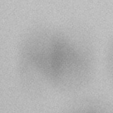
\includegraphics[width=0.185\textwidth]{../../__Images/05/WB_N(20-200)_-0D_to_-4D/wb_N_20-200_Camera-4,00D(lens).png} \\

	\begin{sideways} \parbox[b]{20mm} {Simulation} \end{sideways} &
	
\includegraphics[width=0.185\textwidth]{../../__Images/05/WB_N(20-200)_-0D_to_-4D/wb_N_20-200_Camera-0,00D(simulated).png} &
	
\includegraphics[width=0.185\textwidth]{../../__Images/05/WB_N(20-200)_-0D_to_-4D/wb_N_20-200_Camera-1,00D(simulated).png} &
	
\includegraphics[width=0.185\textwidth]{../../__Images/05/WB_N(20-200)_-0D_to_-4D/wb_N_20-200_Camera-2,00D(simulated).png} &
	
\includegraphics[width=0.185\textwidth]{../../__Images/05/WB_N(20-200)_-0D_to_-4D/wb_N_20-200_Camera-3,00D(simulated).png} &
	
\includegraphics[width=0.185\textwidth]{../../__Images/05/WB_N(20-200)_-0D_to_-4D/wb_N_20-200_Camera-4,00D(simulated).png} \\

	\begin{sideways} \parbox[b]{20mm} {Local~SSIM} \end{sideways} &
	
\includegraphics[width=0.185\textwidth]{../../__Images/05/WB_N(20-200)_-0D_to_-4D/wb_N_20-200_Camera-0,00D(comparison).png} &
	
\includegraphics[width=0.185\textwidth]{../../__Images/05/WB_N(20-200)_-0D_to_-4D/wb_N_20-200_Camera-1,00D(comparison).png} &
	
\includegraphics[width=0.185\textwidth]{../../__Images/05/WB_N(20-200)_-0D_to_-4D/wb_N_20-200_Camera-2,00D(comparison).png} &
	
\includegraphics[width=0.185\textwidth]{../../__Images/05/WB_N(20-200)_-0D_to_-4D/wb_N_20-200_Camera-3,00D(comparison).png} &
	
\includegraphics[width=0.185\textwidth]{../../__Images/05/WB_N(20-200)_-0D_to_-4D/wb_N_20-200_Camera-4,00D(comparison).png} \\
	
	\begin{sideways} \parbox[b]{20mm} {Absolute Difference} \end{sideways} &
	
\includegraphics[width=0.185\textwidth]{../../__Images/05/WB_N(20-200)_-0D_to_-4D/wb_N_20-200_Camera-0,00D(diff).png} &
	
\includegraphics[width=0.185\textwidth]{../../__Images/05/WB_N(20-200)_-0D_to_-4D/wb_N_20-200_Camera-1,00D(diff).png} &
	
\includegraphics[width=0.185\textwidth]{../../__Images/05/WB_N(20-200)_-0D_to_-4D/wb_N_20-200_Camera-2,00D(diff).png} &
	
\includegraphics[width=0.185\textwidth]{../../__Images/05/WB_N(20-200)_-0D_to_-4D/wb_N_20-200_Camera-3,00D(diff).png} &
	
\includegraphics[width=0.185\textwidth]{../../__Images/05/WB_N(20-200)_-0D_to_-4D/wb_N_20-200_Camera-4,00D(diff).png} \\
 
	\end{tabular}
	
	\caption{Comparisons of our simulated results against ground truth obtained with a hyperopic camera. These large images correspond to a Snellen ratio of 20/200. (top row) Images captured using the DSLR camera with extra lenses varying from 0.0 to -4.0 diopters. (second row) Our simulated results. (third row) SSIM metric results. (fourth row) AD metric.}
	\label{fig:comparison_hyperopic_wb}
\end{figure*}